\documentclass[12pt,a4paper]{article}

\usepackage[utf8]{inputenc}
\usepackage[english]{babel}

\usepackage[pdftex]{graphicx}
\usepackage[top=1in, bottom=1in, left=1in, right=1in]{geometry}

\usepackage{listings}

\lstdefinestyle{output}{
	numbers=none, % where to put the line-numbers
	numberstyle=\tiny, % the size of the fonts that are used for the line-numbers     
	backgroundcolor=\color{darkgray},
	basicstyle=\ttfamily\color{white},
	captionpos=b, % sets the caption-position to bottom
	breaklines=true, % sets automatic line breaking
	breakatwhitespace=false,
}


% \linespread{1.06}
% \setlength{\parskip}{10pt plus2pt minus2pt}

\widowpenalty 10000
\clubpenalty 10000

\newcommand{\eat}[1]{}
\newcommand{\HRule}{\rule{\linewidth}{0.5mm}}

\usepackage[official]{eurosym}
\usepackage{enumitem}
\setlist{nolistsep,noitemsep}
\usepackage[hidelinks]{hyperref}
\usepackage{cite}
\usepackage{lipsum}

\usepackage{minted}

\usepackage{amsmath}
\usepackage{fancyvrb}
\usepackage{amsfonts}

\begin{document}

\begin{titlepage}
    \begin{center}

        % Top 
        
\includegraphics[width=0.25\textwidth]{res/NSUT.png}~\\[0.5cm]
        \textsc{\Large Netaji Subhas University of Technology}\\[2cm]

        % Title
        \HRule \\[0.4cm]
        {
        \LARGE
        \textbf{Practical Report}\\[0.4cm]
        \emph{Microprocessors and Microcontrollers}\\[0.4cm]
        }
        \HRule \\[1.5cm]



        % Author
        { \large
        Kushagra Lakhwani \\[0.1cm]
        \texttt{2021UCI8036}\\[0.5cm]
        Computer Science Engineering (Internet of Things)\\[0.1cm]
        \textit{Semester 3} \\[0.1cm]
        }

        \vfill

        \textsc{\large Department of Computer Science \& Engineering}\\[0.4cm]


        % Bottom
        {\large \today}

    \end{center}
\end{titlepage}

\newpage

\begin{abstract}
    The lab project report \textit{Database Management System} is submitted by \textit{Kushagra Lakhwani}\cite{Kushagra} (Roll No. 2021UCI8026).
    The report is submitted to the \textit{Mr. Vishal Gupta}, Department of Computer Science and Engineering, Netaji Subhas University of Technology in the fulfillment of the requirements for the course of \textit{Database Management System} (semester 3).

\end{abstract}


\pagebreak

\tableofcontents
\addtocontents{toc}{\protect\thispagestyle{empty}}
\newpage
\setcounter{page}{1}


\newcommand { \inputsql } [1] {
	\inputminted[autogobble,breaklines,breaklines,frame=single,framesep=5pt,fontsize=\footnotesize]{sql}{sql/#1.sql}
}

\newcommand { \key } [1] {\underline{\texttt{#1}}}

\newenvironment{sqlSchema}[2][h!bp]
{
	\VerbatimEnvironment
	\label{#2}%
	\begin{listing}[#1]% which is h!bp
		\centering
		\begin{minted}[autogobble, breaklines, breaklines, frame=single, framesep=5pt, escapeinside=||, fontsize=\footnotesize ]{sql}%
}
{ \end{minted}\end{listing} }

\newenvironment{sqlQuery}[2][h!bp]
{
	\VerbatimEnvironment
	\label{#2}%
	\centering
	\begin{minted}[ autogobble,breaklines,breaklines,frame=single,framesep=5pt,escapeinside=||,fontsize=\footnotesize ]{sql}%
}
{ \end{minted} }

\section{Sailors}

\subsection{Schema}

Consider the following relational schema:


\begin{sqlSchema}{sea}

      SAILORS (|\key{sid}|, sname, rating, date_of_birth)

      BOATS (|\key{bid}|, bname, color)

      RESERVES (|\key{sid, bid, date, time\_slot}|)

\end{sqlSchema}


\subsection{Queries}

\begin{enumerate}
      \item  Find sailors who've reserved at least one boat
            \begin{enumerate}
                  \item Relational Algebra
                        \begin{equation*}
                              \pi_{sid, sname}(SAILORS \bowtie RESERVES))
                        \end{equation*}

                  \item  SQL \linebreak \inputsql{01}
            \end{enumerate}
            \vspace{1cm}

      \item Find names of sailors who've reserved a red or a green boat in the month of March.
            \begin{enumerate}
                  \item Relational Algebra
                        \begin{multline*}
                              \pi_{sname}(SAILORS \bowtie RESERVES \bowtie BOATS) \bowtie \\
                              \sigma_{\text{bname} = \text{red} \lor \text{bname} = \text{green}}(\sigma_{\text{date} = \text{March}}(BOATS \bowtie RESERVES))
                        \end{multline*}

                  \item  SQL
                        \begin{sqlQuery}{sea2}
                            SELECT sname
                            FROM SAILORS
                            WHERE sid IN
                                (SELECT sid
                                FROM RESERVES
                                WHERE bid IN
                                    (SELECT bid
                                    FROM BOATS
                                    WHERE bname = 'red' OR bname = 'green')
                                AND (SELECT extract(month FROM date) FROM RESERVES) = 3)
                    \end{sqlQuery}

            \end{enumerate}

      \item  Find names of sailors who've reserved a red and a green boat

            \begin{enumerate}
                  \item Relational Algebra
                        \begin{multline*}
                              \pi_{sname}(SAILORS \bowtie RESERVES \bowtie (\sigma_{\text{color} = red}(BOATS))) \; \cap  \\
                              \pi_{sname}(SAILORS \bowtie RESERVES \bowtie (\sigma_{\text{color} = green}(BOATS)))
                        \end{multline*}

                  \item SQL
                        \begin{sqlQuery}{sea3}
                    SELECT DISTINCT S1.sname
                    FROM SAILORS S1, RESERVES R1, BOATS B1,
                    RESERVES R2, BOATS B2
                    WHERE S1.sid = R1.sid 
                        AND R1.bid = B1.bid
                        AND S1.sid = R2.sid 
                        AND R2.bid = B2.bid
                        AND B1.color = "red" 
                        AND B2.color = "green";
                \end{sqlQuery}
            \end{enumerate}

      \item Find \textsc{sid} of sailors who have \underline{not} reserved a boat after Jan 2018.

            \begin{enumerate}
                  \item Relational Algebra

                        \begin{equation*}
                              \pi_{\text{sid}} - \pi_{\text{sid}}(SAILORS \bowtie \sigma_{\text{date\_of\_birth}\; >\; \text{Jan 2018}}(RESERVES))
                        \end{equation*}

                  \item SQL
                        \begin{sqlQuery}{sea4}
                    SELECT sid FROM SAILORS 
                    WHERE sid NOT IN 
                        (SELECT sid FROM RESERVES 
                        WHERE date_of_birth > "2018-01-01")
                    \end{sqlQuery}

            \end{enumerate}

      \item  Find sailors whose rating is greater than that of all the sailors named "John"
            \begin{enumerate}
                  \item Relational Algebra

                        \begin{multline*}
                              \pi_{\text{sid}, \text{sname}}(SAILORS) \\
                              - \pi_{S_2.\text{sid},S_2.\text{sname}}(\sigma_{S_2.\text{rating} < S.\text{rating}}(\rho_{S_2}(SAILORS)\times \rho_S(SAILORS)))
                        \end{multline*}

                  \item SQL

                        \begin{sqlQuery}{sea5}
                        SELECT sid, sname FROM SAILORS S1
                        WHERE S1.rating > ALL
                                (SELECT S2.rating FROM SAILORS S2
                                WHERE S2.sname = "John")
                    \end{sqlQuery}

            \end{enumerate}

      \item Find sailors who've reserved all boats

            \begin{enumerate}
                  \item Relational Algebra
                        \begin{equation*}
                              \pi_{\text{sid}, \text{sname}}(\pi_{\text{sid}, \text{bid}}(RESERVES) \div \pi_{\text{bid}}(BOATS)) \\
                              \bowtie SAILORS
                        \end{equation*}
                        \pagebreak
                  \item SQL
                        \begin{sqlQuery}{sea6}
                        SELECT S.sid, S.sname
                        FROM SAILORS S
                        WHERE NOT EXISTS
                              (SELECT B.bid
                              FROM BOATS B
                              WHERE NOT EXISTS
                                    (SELECT R.sid, R.bid
                                    FROM RESERVES R
                                    WHERE R.sid = S.sid
                                          AND R.bid = B.bid))
                  \end{sqlQuery}
            \end{enumerate}

      \item Find name and age of the oldest sailor(s)

            \begin{enumerate}
                  \item Relational Algebra
                        \begin{multline*}
                              \pi_{\text{sname}, \text{age}}(\pi_{sid}(SAILORS) - \\
                              \pi_{S_2.sid}(\sigma_{S_2.\text{age} < S.\text{age}}(\rho_{S_2}(SAILORS) \times \rho_{S}(SAILORS)))) \\
                              \bowtie SAILORS
                        \end{multline*}
                  \item SQL

                        \begin{sqlQuery}{sea7}
                        SELECT sname, age FROM SAILORS S1
                        WHERE S1.date_of_birth > ALL
                                (SELECT S2.date_of_birth FROM SAILORS S2)
                        \end{sqlQuery}

            \end{enumerate}

      \item  Find the age of the youngest sailor for each rating with at least 2 such sailors

            \begin{enumerate}
                  \item Relational Algebra
                        \begin{multline*}
                              \pi_{\text{rating}, \text{minage}}(\sigma_{\text{no\_of\_sailors} > 1} \\
                              (\rho_{r (\text{rating}, \text{no\_of\_sailors}, \text{minage}) \; \mathcal{F} \; (\text{rating}, count(\text{sid}), min(\text{age}))} \\
                              (SAILORS)))
                        \end{multline*}
                  \item SQL

                        \begin{sqlQuery}{sea8}
                              SELECT rating, age FROM SAILORS S1
                              WHERE S1.date_of_birth > ALL AS minage
                                          (SELECT S2.date_of_birth FROM SAILORS S2
                                          WHERE S2.rating = S1.rating)
                              GROUP BY rating
                              HAVING COUNT(*) >= 2
                        \end{sqlQuery}
            \end{enumerate}

\end{enumerate}


\pagebreak

\section{Customers}

\subsection{Schema}

Consider the following relational schema:

\begin{sqlSchema}{customers}

	CUSTOMERS (|\key{cust\_num}|, |\text{cust\_lname}|, |\text{cust\_fname}|, |\text{cust\_balance}|)

	PRODUCT (|\key{prod\_num}|, |\text{prod\_name}|, price)

	INVOICE (|\key{inv\_num, prod\_num, cust\_num, inv\_date}|, |\text{unit\_sold}|, |\text{inv\_amount}|)

\end{sqlSchema}

\subsection{Table Definitions}

\begin{enumerate}[label=\alph*)]
	\item Create the tables for the schema

	      \inputsql{customers}

	      \begin{lstlisting}[style=output]
practicals=# \dt
    List of relations
Schema |   Name   | Type  |  Owner
--------+----------+-------+----------
public | customers | table | postgres
public | invoice   | table | postgres
public | product   | table | postgres
(3 rows)
          \end{lstlisting}

	\item Insert the following tuples into the tables

	      \inputsql{customers_data}

\end{enumerate}

\subsection{Queries}

Write SQL queries and relational algebraic expression for the following:

\begin{enumerate}
	\item Find the names of the customer who have purchased no item. Set default value of cust\_balance as 0 for
	      such customers.

	      \begin{enumerate}
		      \item Relational Algebra

		            \begin{equation*}
			            \pi_{\text{cust\_lname} + " " + \text{cust\_fname}}(\sigma_{\text{cust\_balance} = 0} (CUSTOMERS))
		            \end{equation*}
		            \pagebreak

		      \item SQL

		            \begin{sqlQuery}{customers1}
                        SELECT concat(cust_lname , ' ' , cust_fname) as name
                        FROM CUSTOMERS
                        WHERE cust_balance = 0;
                    \end{sqlQuery}

		      \item Output

		            \begin{lstlisting}[style=output]
practicals=# \i /home/sql/customers1.sql
    name    
------------
 Smith John
 Smith Mary
(2 rows)
                    \end{lstlisting}

	      \end{enumerate}

	\item Write the trigger to update the \textsc{CUST\_BALANCE} in the CUSTOMER table when a new invoice record
	      is entered for the customer.


	      \begin{sqlQuery}{customers2}
                CREATE TRIGGER update_cust_balance
                AFTER INSERT ON INVOICE
                FOR EACH ROW
                BEGIN
                    UPDATE CUSTOMERS
                    SET cust_balance = cust_balance + NEW.inv_amount
                    WHERE cust_num = NEW.cust_num;
                END;
        \end{sqlQuery}


	\item Find the customers who have purchased more than three units of a product on a day.

	      \begin{enumerate}
		      \item Relational Algebra

		            \begin{multline*}
			            \pi_{\text{cust\_lname} + " " + \text{cust\_fname}} (\sigma_{\text{unit\_sold} \geq  3} \\
			            (CUSTOMER \bowtie \sigma_{\text{unit\_sold}}\\
			            ({}_{\text{cust\_num, inv\_date} > \text{prod\_num}} \; \mathcal{F}_{\; sum(\text{unit\_sold})} (INVOICE))))
		            \end{multline*}

		      \item SQL

		            \begin{sqlQuery}{customers3}
                        SELECT concat(cust_lname , ' ' , cust_fname) as name
                        FROM CUSTOMERS
                        WHERE cust_num IN
                        (
                            SELECT cust_num
                            FROM INVOICE
                            GROUP BY cust_num, inv_date, prod_num
                            HAVING sum(unit_sold) >= 3
                        );
                    \end{sqlQuery}
		            \pagebreak

		      \item Output

		            \begin{lstlisting}[style=output]
practicals=# \i /home/sql/customers3.sql
    name    
------------
 Smith John
 Jones Mary
(2 rows)
                    \end{lstlisting}

	      \end{enumerate}

	\item Write a query to illustrate Left Outer, Right Outer and Full Outer Join.

	      \begin{enumerate}
		      \item Left Outer Join
		            \begin{equation*}
			            CUSTOMER ]\bowtie INVOICE
		            \end{equation*}

		            \begin{sqlQuery}{customer4a}
											SELECT CONCAT(C.cust_fname, c.cust_lname) as name,
											LEFT JOIN INVOICE i
											ON C.cust_num=i.cust_num
										\end{sqlQuery}

		      \item Right Outer Join

		            \begin{equation*}
			            CUSTOMER \bowtie[ INVOICE
		            \end{equation*}

		            \begin{sqlQuery}{customer4b}
											SELECT CONCAT(C.cust_fname, c.cust_lname) as name,
											RIGHT JOIN INVOICE i 
											ON C.cust_num=i.cust_num
										\end{sqlQuery}

		      \item Full Outer Join

		            \begin{equation*}
			            CUSTOMER ]\bowtie[ INVOICE
		            \end{equation*}

		            \begin{sqlQuery}{customer4c}
                    SELECT CONCAT(C.cust_fname, " ", C.cust_lname) as name
                    LEFT JOIN INVOICE i
                    ON C.cust_num=i.cust_num
                    UNION
                    SELECT CONCAT(C.cust_fname, " ", C.cust_lname) as name, i.inv_amount
                    RIGHT JOIN INVOICE i
                    ON C.cust_num=i.cust_num
                    \end{sqlQuery}

	      \end{enumerate}
	      \pagebreak

	\item Count number of products sold on each date.

	      \begin{enumerate}
		      \item Relational Algebra

		            \begin{equation*}
			            \pi_{\text{inv\_date}, sum(\text{unit\_sold})}({}_{\; \text{inv\_date}} \; \mathcal{F}_{\; sum(\text{unit\_sold})} (INVOICE))
		            \end{equation*}

		      \item SQL

		            \begin{sqlQuery}{customers5}
                        SELECT inv_date, sum(unit_sold)
                        FROM INVOICE
                        GROUP BY inv_date
                    \end{sqlQuery}

		      \item Output

		            \begin{lstlisting}[style=output]
practicals=# SELECT inv_date, sum(unit_sold)
    FROM INVOICE
    GROUP BY inv_date;
  inv_date  | sum 
------------+-----
 2015-10-01 |  10
 2015-07-01 |   7
 2015-03-01 |   3
 2015-02-01 |   2
 2015-01-01 |   8
 2015-06-01 |  14
 2015-05-01 |   5
 2015-11-01 |   1
 2015-04-01 |  13
(9 rows)
                \end{lstlisting}


	      \end{enumerate}

	\item As soon as customer balance becomes greater than Rs. 100,000, copy the customer\_num in new table
	      called "GOLD\_CUSTOMER"

	      \begin{enumerate}
		      \item Create table GOLD\_CUSTOMER

		            \begin{sqlQuery}{customers6a}
                        CREATE TABLE GOLD_CUSTOMER
                        (
                            cust_num int,
                            PRIMARY KEY (cust_num),
                            FOREIGN KEY (cust_num) REFERENCES CUSTOMERS (cust_num)
                        )
                    \end{sqlQuery}
		            \pagebreak

		      \item Create a trigger to update the GOLD\_CUSTOMER table when a new invoice record is entered for the customer.

		            \begin{sqlQuery}{customers6b}
                        CREATE TRIGGER update_gold_customer
                        AFTER INSERT ON INVOICE
                        FOR EACH ROW
                        BEGIN
                            IF NEW.cust_balance > 100000 
                            AND NEW.cust_num NOT IN (SELECT cust_num FROM GOLD_CUSTOMER) THEN
                                INSERT INTO GOLD_CUSTOMER VALUES (NEW.cust_num);
                            END IF;
                        END                        
                    \end{sqlQuery}

	      \end{enumerate}

	\item Add a new attribute CUST\_DOB in customer table

	      \begin{sqlQuery}{customers7}
            ALTER TABLE CUSTOMERS
            ADD COLUMN cust_dob date
          \end{sqlQuery}

\end{enumerate}

\section{Case Study: Library Management System}

\subsection{Introduction}

Online Library Management System is a system which
maintains the information about the books present in the
library, their authors, the members of library to whom
books are issued, library staff and all.

This is very difficult to organize manually.
Maintenance of all this information
manually is a very complex task.
Owing to the advancement of technology, organization of an Online Library becomes much simple.

The Online Library Management has been designed to computerize and
automate the operations performed over the information
about the members, book issues and returns and all other
operations. This computerization of library helps in many
instances of its maintenances. It reduces the workload of
management as most of the manual work done is reduced.

\subsection{Objective}

The main objective of this project is to develop a system that
will help in maintaining the information about the books present in the library, their authors, the members of library to whom books are issued, library staff and all.

The library management system keeps track of reader with the following considerations:

\begin{enumerate}
    \item The system keeps track of the staff with a single point
          authentication system comprising login ID and password.
    \item Staff maintains the book catalog with its ISBN, Book title, price(in INR), category(novel, general, story), edition, author
          Number and details.
    \item A publisher has publisher ID, Year when the book was
          published, and name of the book.
    \item Readers are registered with their user ID, email,
          name (first name, last name), Phone no (multiple entries allowed), communication address. The staff keeps track of readers.

    \item Readers can return/reserve books that stamps with issue
          date and return date. If not returned within the prescribed time period, it may have a due date too.
    \item Staff also generate reports that have readers ID, registration number of report, book number and return/issue info.
\end{enumerate}

\subsection{Design}

The following are the entities of the system:

\subsubsection{Entities}

\begin{itemize}
    \item \textbf{Book}

          It has authno, isbn number, title, edition, category,
          price. ISBN is the Primary Key for Book Entity.
    \item \textbf{Reader}

          It has UserId, Email, address, phone no, name.
          Name is composite attribute of firstname and lastname. Phone No. is multivalued attribute. UserId is the Primary Key for Readers
          entity.
    \item \textbf{Publisher}

          It has PublisherID, Year of publication,
          name. PublisherID is the Primary Key.
    \item \textbf{Authentication System}

          It has LoginID and password
          with LoginID as Primary Key.
    \item \textbf{Reports}

          It has UserId, Reg\_no, Book\_no, Issue/Return
          date. Reg\_no is the Primary Key of reports entity.
    \item \textbf{Staff}

          It has name and staff\_id with staff\_id as Primary Key.
    \item \textbf{Reserve/Return Relationship Set}

          It has three attributes:
          Reserve date, Due date, Return date.
\end{itemize}

The relationships between the entities are as follows:

\subsubsection{Relationships}

\begin{itemize}
    \item A reader can reserve N books, but one book can be reserved by
          only one reader. The relationship 1:N.
    \item A publisher can publish many books, but a book is published by
          only one publisher. The relationship 1:N.
    \item Staff keeps track of readers. The relationship is M:N.
    \item Staff maintains multiple reports. The relationship 1:N.
    \item Staff maintains multiple Books. The relationship 1:N.
    \item Authentication system provides login to multiple staffs. The relation is 1:N.

\end{itemize}

\subsubsection{ER Diagram}

\begin{figure}[ht]
    \centering
    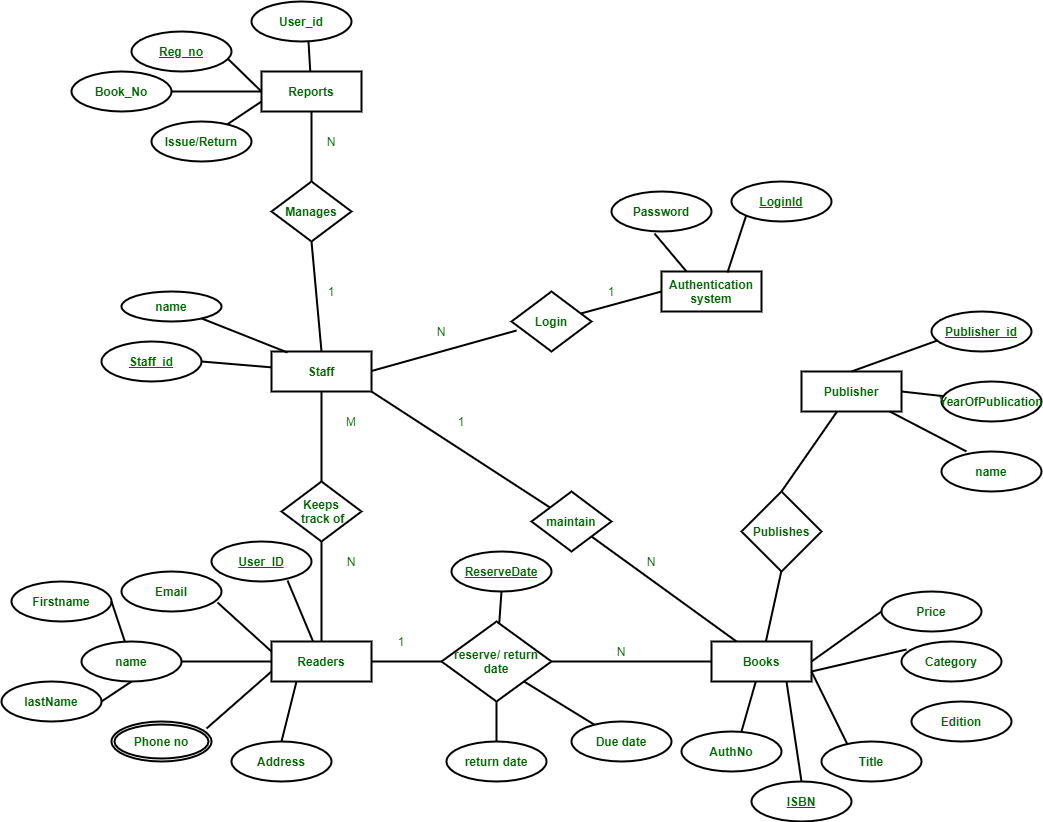
\includegraphics[width=0.9\textwidth]{res/libraryER.png}
    \caption{ER Diagram}
    \label{fig:er-diagram}
\end{figure}

\bibliographystyle{ieeetr}
\bibliography{refs}

\end{document}
